\newcommand{\galextable}{\begin{tabular}{|c|D{.}{.}{3.2}|}
\hline
\multicolumn{1}{|c|}{\textbf{CPU time (per image)}} &\multicolumn{1}{c|}{\textbf{Percentage of images recognized}} \\
\hline
\makebox[\pointonesec][r]{$1$ s} & 74.46 \\
\makebox[\pointonesec][r]{$10$ s} & 93.56 \\
\makebox[\pointonesec][r]{$100$ s} & 98.95 \\
\makebox[\pointonesec][r]{$1000$ s} & 99.74 \\
\hline
\end{tabular}
}
\newcommand{\galexcputimefig}{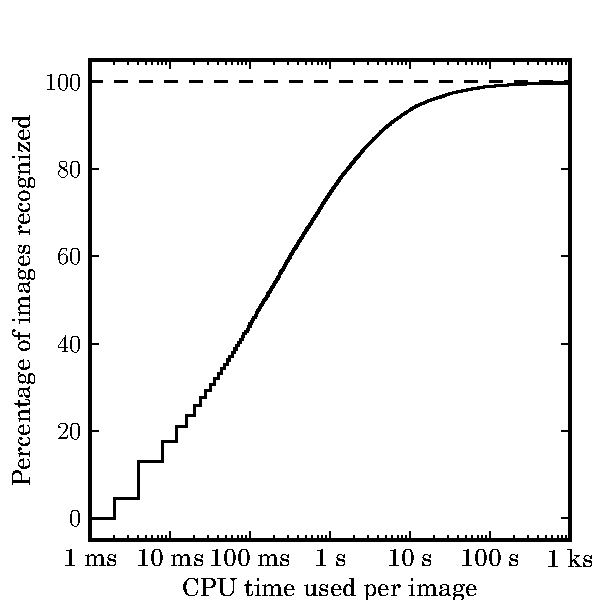
\includegraphics[width=1.000000\figunit]{galex-cputime}}
\newcommand{\galexindexidfig}{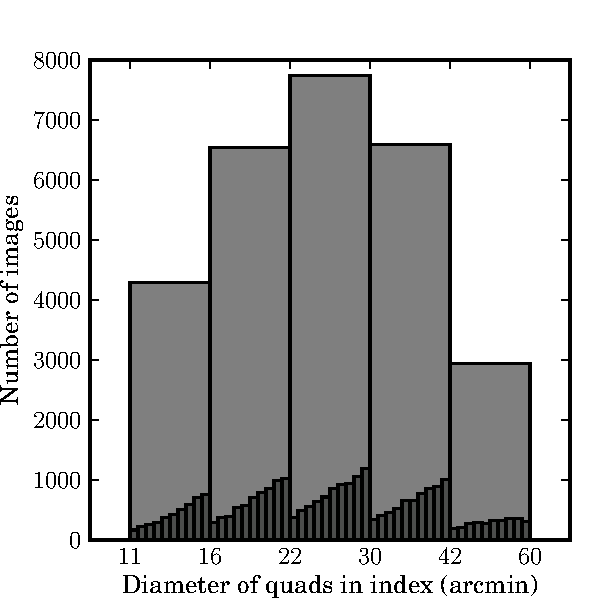
\includegraphics[width=1.000000\figunit]{galex-indexid}}
